% 独自のコマンド

% ■ アブストラクト
%	\begin{jabstract} ~ \end{jabstract}	:日本語のアブストラクト

% ■ 謝辞
%	\begin{acknowledgment} ~ \end{acknowledgment}

% ■ 文献リスト
%	\begin{bib}[100] ~ \end{bib}

% styファイルは同ディレクトリにおいておけば,latexmkrcの設定をいじらなくても上手くいくらしい
\newif\ifjapanese

\japanesetrue	% 論文全体を日本語で書く(英語で書くならコメントアウト)

\ifjapanese
	\documentclass[12pt]{jreport}
	\renewcommand{\bibname}{参考文献}
	\newcommand{\acknowledgmentname}{謝辞}
\else
	\documentclass[11pt]{report}
	\newcommand{\acknowledgmentname}{Acknowledgment}
\fi
\usepackage{ascmac}
\usepackage[dvipdfmx]{graphicx}
\usepackage{multirow}
\usepackage{ylab_thesis} % このスタイルファイルが同じディレクトリにあることを確認すること
\usepackage{layout}

% \documentclass[dvipdfmx]{jsarticle}
% \usepackage[dvipdfmx]{graphicx}
\usepackage{amsmath, amssymb}
\usepackage{mathtools}
\usepackage{here}

% \bindermode	% バインダ用余白設定

% 日本語情報(必要なら)
\jclass	{卒業論文}							% 論文種別
\jtitle		{オープンセット環境下におけるレーダ心拍信号を用いた深層学習による人物識別}					% タイトル。改行する場合は\\を入れる
\juniv		{慶 應 義 塾 大 学}					% 大学名
\jfaculty	{理 工 学 部 情 報 工 学 科}				% 学部、学科
\jlab		{大 槻 研 究 室}						% 研究室
\jauthor	{権 藤 陸}						% 著者
\jid		{61908013}						% 学籍番号
\jadvisor	{大 槻 知 明}{教 授}					% 指導教官、形式は『{名前}{肩書}』
\jsubmit	{令和 5 年 2 月 3 日}
\jhyear		{5}							% 平成○年度
\jsyear		{2023}							% 西暦○年度
\jkeyword	{キーワード1,キーワード2,キーワード3}		% 論文のキーワード


\begin{document}

\jmaketitle		% 表紙(日本語)、不要ならコメントアウト

%%% アブストラクト
\begin{jabstract}

テンプレートの説明を,テンプレート自身を使って説明する.これは卒業論文のための\LaTeX テンプレートで,本当は卒業論文のために作成したものだけどでもたぶんきっと修士論文にも使えると思う.

この部分には一般には論文のアブストラクトを書く.日本語のアブストラクトを書きたいなら,\verb|\begin{jabstract}| と \verb|\end{jabstract}| の間に文章を書けば,今のこのページのように体裁が勝手に整って出力される.英語のアブストラクトは \verb|\begin{eabstract}| と \verb|\end{eabstract}| の間に書けば,次ページのような体裁で出力される.

両方を書けば,日本語と英語の両方のアブストラクトが並んで出力される(この文書はサンブルなので両方書いてある).ページ順序は,コマンドを書いた順序の通り.どちらか一方のみを出力したい場合は,不要な方をコマンド自体を含め削除する.

このあたりの詳細もあとで書く.基本的には,{\tt main.tex}を上から順にいじっていけばできるはず.

(2018/11 中村追記) ファイル分割を廃止し{\tt main.tex}に統一している.

\end{jabstract}

\tableofcontents	% 目次
\listoffigures		% 表目次
\listoftables		% 図目次

\pagenumbering{arabic}

\chapter{序論}
\label{chap_introduction}

論文は序論のようなもので始める.タイトルは序論でも序言でもはじめにでもいいけど,『序論』で始めたら『結論』で終わり,『序言』で始めたら『結言』で終わるようにする.『はじめに』なら『おわりに』で終わる.『序論』で始まって『おわりに』でおわるとか,そういうちぐはぐなのはだ.

ここでは序論として書く.序論では,研究の背景やら目的やらを書くのが普通.今はテンプレートの説明なので,大して書くことは無い.

このような高齢者の家庭内事故の現状を踏まえると,高齢者が最も遭遇しやすい事故は屋内での転倒・転落事故と推定され,
これらの異常事態の迅速かつ高精度な検知が今後の見守りシステムにおける重要課題と言える.

\section{背景}

卒論向けテンプレ

\section{本文書の構成}

第1章の最後は,文書全体の構成を大まかに書くとよいらしい.

第\ref{chap_introduction}章では本テンプレートの概要みたいなものを書いた.



\chapter{ドップラーレーダの原理}
\begin{equation*} f_{\mathrm{ Doppler}} = \mp \frac {4 \pi vt}{\lambda } \times \frac {1}{2 \pi t} = \mp \frac {2v}{\lambda },\tag{1}\end{equation*}

\begin{equation*} B(t)=\cos \left({\theta +\frac {4\pi x_{h}(t)}{\lambda }+\Delta \Phi (t)}\right),\tag{2}\end{equation*}

\begin{align*} I(t)=&\cos \left({\theta +\frac {\pi }{4}+\frac {4\pi x_{h}(t)}{\lambda }+\Delta \Phi (t)}\right), \tag{3}\\ Q(t)=&\cos \left({\theta -\frac {\pi }{4}+\frac {4\pi x_{h}(t)}{\lambda }+\Delta \Phi (t)}\right).\tag{4}\end{align*}

\chapter{関連研究}

\chapter{従来法}
本章では,本研究と同様に心拍信号を用いて人物識別を行った研究について述べる.

\section{心拍信号のスペクトログラムを用いた深層学習による人物識別\cite{paper:HeartID}}
\subsection{手法}
24 GHz?ドップラーレーダを用いて取得した心拍信号に対し,STFT(Short Time Fourier Transform)を実行して得たスペクトログラムが入力である.
そして,時間軸と周波数軸で表現された特徴量をAlexNetを基にしたDCNN(Deep Convolutional Neural Network)で抽出し,4人の人物識別をクローズセット環境下で行った.
\cite{paper:HeartID}では,人物識別における深層学習の有用性を示している.比較手法として,SVM(Support Vector Machine), Naive Bayes, そしてそれらを組み合わせた手法のSVM-Bayesが挙げられており,用いられた手動の特徴量は以下の三種である.一つ目は,心拍信号の周期,二つ目は心拍信号のエネルギー,三つ目はドップラー信号の帯域幅である.

\subsection{実験結果}
先ほども触れたとおり,DCNNを用いた手法は伝統的な機械学習手法の精度を上回った.表\ref{table:HeartID}に各手法ごとの4人の被験者のクローズセット環境下における精度の比較を示す.

\begin{table}[H]
\caption{各手法における4人の被験者のクローズセット環境下における精度の比較}
\centering
\begin{tabular}{cc}
\hline
手法 & 精度 \\
\hline
DCNN & 98.5\% \\
SVM-Bayes & 91.25\% \\
SVM & 88.75\% \\
Naive Bayes & 80.75\% \\
\hline
\end{tabular}
\label{table:HeartID}
\end{table}

\section{心拍信号を基にした,双極子深層学習モデルによるオープンセット環境下における人物識別\cite{paper:HeartSignature}}
\subsection{手法}
6ポートCW(Continuous Wave)レーダを用いて取得した心拍信号が入力であり,使用されたデータセットは本研究でも評価した公開データセットである.
手動の特徴量ではなく,1次元のCNN(Convolutional Neural Network)を用いて特徴量を抽出して分類に使用する.
それらの特徴量はユークリッド距離をベースとした損失関数を通してネットワークに学習される.各クラスにそれぞれ双極子が設定されており,損失関数はそれらの双極子とマッピングされた特徴量との距離が主な要素となっている.
これらの損失関数はクラス内のクラスタリング,クラス間の分離をどちらも強化する.それによって,特徴量空間上でクラスがより分離可能な分布となる.
また,双極子自体の分布も学習により調整され,抽出された特徴量とは敵対的学習の形をとる.識別の際にも双極子は使用され,ある心拍セグメントの潜在表現がクラスAの正極から閾値以上の距離があるか,負極から閾値以下の距離に存在する場合に,その心拍セグメントはクラスAと識別される.以上のように提案されたアーキテクチャは,オープンセット環境下で,学習に使用していない未知のデータに対しても対応できるように考案されたものである.

\subsection{実験結果}
実験では,クローズセット環境下とオープンセット環境下の2つの状態で評価が行われた.
図\ref{fig:HeartSignature}に結果を示す.

\begin{table}[H]
\caption{クローズ/オープンセットにおける精度}
\centering
\begin{tabular}{ccc}
\hline
環境 & 人数 & 精度 \\
\hline
クローズセット & 30 & 99.17\% \\
オープンセット & 15/15 & 93.57\% \\
\hline
\end{tabular}
\end{table}

\section{心拍信号を基にした,転移学習とアンサンブル学習を用いたオープンセット環境下における人物識別\cite{paper:Xing}}

\chapter{提案法}
提案法のアルゴリズムを図\ref{fig:proposed_method}に示す.
本提案では,6ポートのドップラーレーダで取得したI/Qデータを用いた.
I/Qデータには心拍信号や呼吸信号に起因する胸壁の変位以外に,体動やI/Qチャネル間の振幅と位相の不均衡に起因するノイズが含まれている.

まずI/Qチャネル間の不均衡補償を行うため,楕円フィッティングを用いた.I/Qデータが推定された理想的な楕円に近似されることで,より正確な変位信号を得ることができる\cite{paper:ellipse1}\cite{paper:ellipse2}.
そして,補償されたI/Qデータにアークタンジェント復調を施すことで,アンラップされた位相値を得ることができる.

そして位相値の変化を$\Delta \sigma$,周波数を$f$, 光速を$c$とすれば,胸壁の相対距離の変化$\Delta x$は,次式のように計算できる.

\begin{equation}
	\Delta x = \frac{\Delta \sigma}{2 \pi} \cdot \frac{\lambda}{2}
	\end{equation}

本稿では,ノイズの少ないデータセットとノイズの多いデータセットの2つを使用するが,後者の場合にはこのあとウェーブレット再構成を行う.
胸壁変位信号には,レーダのキャリブレーションを含む高周波ノイズが含まれている.信号に対しウェーブレット変換を行うと,ウェーブレット係数を得ることができる.そしてそれらの係数に適切な閾値処理を施したあとに逆ウェーブレット変換を行うことで,ノイズが除去された信号を得ることが可能である.今回はレベルを8,マザーウェーブレットをDaubechies8とした.閾値処理では,最も高周波な成分を0として取り除いた.

所望の信号を得られたら,次にセグメンテーションを行う.詳細な諸元については第6章で述べるが,セグメントのウィンドウ長は5秒,隣り合うセグメントとのオーバーラップは1.5秒とした.

\begin{figure}[H]
\begin{center}
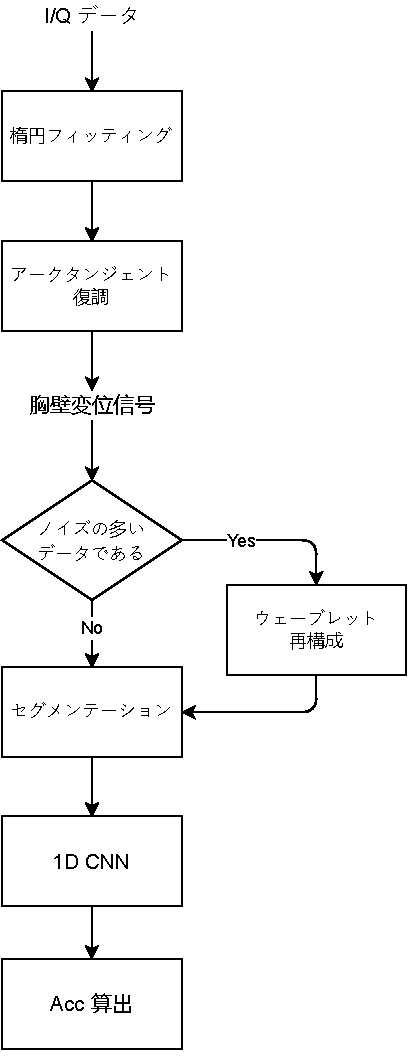
\includegraphics[width=0.5\linewidth]{./fig/proposed_method.pdf}
\end{center}
\caption{提案法のアルゴリズム}
\label{fig:proposed_method}
\end{figure}

\chapter{実験評価}
\section{ノイズの少ないデータセットについて}
エルランゲン大学病院で収集された30人の被験者に対するデータセット
\subsection{クローズセット環境}
\subsubsection{実験諸元}
\subsubsection{実験結果}
\subsection{オープンセット環境}
\subsubsection{実験諸元}
\subsubsection{実験結果}


\section{ノイズの多いデータセットについて}
慶應大学病院で収集された12人の被験者に対するデータセット
\subsection{クローズセット環境}
\subsubsection{実験諸元}
\subsubsection{実験結果}
\subsection{オープンセット環境}
\subsubsection{実験諸元}
\subsubsection{実験結果}


\chapter{結論}

\chapter{それ以降の書き方}
\section{構成}
基本的に,以下のような流れになるが,これに従う必要はない.
おそらく{\tt subsection}や{\tt subsubsection}でまとめる場合もあるはず.

\begin{enumerate}
	\item 序論
	\item 関連研究
	\item 従来法
	\item 提案法
	\item 実験・評価
	\item 考察
	\item 結論
	\item 参考文献
\end{enumerate}

わからなければ,今までサーベイした国際会議の論文や,先輩の卒業論文を参考にしよう.
分量としては,一般的な国内研究会・国際会議のスタイル (2カラム10ポイント) で5・6枚程度の論文の場合,卒論のスタイルファイルに当てはめると40枚超にはなるはず.

\section{参考文献について}
このテンプレ中では{\tt thebibliography}を使用しているが,BibTexのほうが使いやすいと思う場合は変更すること.
引用フォーマットに関しては,IEEEのフォーマット{\tt IEEETran}に筆者は合わせた.

% 謝辞
\begin{acknowledgment}

謝辞には,お世話になった先生,先輩,後輩,友人など,感謝の気持ちを書く.論文が『である』調でも,謝辞だけは『ですます』調で書くひともいる.

\end{acknowledgment}

% 参考文献
\begin{bib}[100]

% \bibitem{参照用名称}
%   著者名: 
%   \newblock 文献名,
%   \newblock 書誌情報,出版年.

\bibitem{hoge09}
  ほげ山太郎,ほげ山次郎:
  \newblock ほげほげ理論のHCI分野への応用,
  \newblock ほげほげ学会論文誌,Vol.31,No.3,pp.194-201,2009.

\bibitem{hoge08}
  Taro Hogeyama, Jiro Hogeyama:
  \newblock The Theory of Hoge,
  \newblock {\it The Proceedings of The Hoge Society}, 2008.

  \bibitem{paper:HeartID}
  AAA

\bibitem{paper:HeartSignature}
  Yang Bajiu, 

\bibitem{paper:Xing}
  Zelin Xing, 
	
\bibitem{paper:ellipse1}
  Aditya Singh, Xiaomeng Gao, Ehsan Yavari, Mari Zakrzewski, Xi Hang Cao, Victor M. Lubecke, Olga Boric-Lubecke
  \newblock Data-Based Quadrature Imbalance Compensation for a CW Doppler Radar System
  \newblock {\it IEEE Transactions on Microwave Theory and Techniques}, Vol.61, No.4, pp.1718-1724, 2013.

\bibitem{paper:ellipse2}
  Mari Zakrzewski, Aditya Singh, Ehsan Yavari, Xiaomeng Gao, Olga Boric-Lubecke, Jukka Vanhala, Karri Palovuori
  \newblock Quadrature Imbalance Compensation With Ellipse-Fitting Methods for Microwave Radar Physiological Sensing
  \newblock {\it IEEE Transactions on Microwave Theory and Techniques}, Vol.62, No.6, pp.1400-1408, 2014.

\end{bib}

\appendix
% 付録
\chapter{付録の例}

付録を無理矢理出力させるため,てきとうなことを書く

\section{付録1}

コマンドは本文と一緒.

\subsection{あの}

あのイーハトーヴォのすきとおった風,夏でも底に冷たさをもつ青いそら,うつくしい森で飾られたモリーオ市,郊外のぎらぎらひかる草の波.

\section{なにか}

あのイーハトーヴォのすきとおった風,夏でも底に冷たさをもつ青いそら,うつくしい森で飾られたモリーオ市,郊外のぎらぎらひかる草の波.

\subsection{foo}

あのイーハトーヴォのすきとおった風,夏でも底に冷たさをもつ青いそら,うつくしい森で飾られたモリーオ市,郊外のぎらぎらひかる草の波.

\end{document}

